% Mid-Semester Report -- NeurIPS 2025 LaTeX Format
\documentclass{article}
\usepackage[preprint]{neurips_2025}

\usepackage[utf8]{inputenc}
\usepackage[T1]{fontenc}
\usepackage{amsmath,amssymb,amsfonts}
\usepackage{booktabs}
\usepackage{graphicx}
\usepackage{float}
\usepackage{hyperref}
\usepackage{url}

% Replace the "Preprint." footer string from the NeurIPS style
% with a course-appropriate label for this mid-semester report.
\makeatletter
\renewcommand{\@noticestring}{NS26Z171 Mid-ject Report, IIT Madras}
\makeatother

\title{Auditing Copyright Protection in Language Models:\\Can We Verify Near-Access Freeness Guarantees?\\[4pt]\normalsize \textit{Mid-Semester Project Report}}

\author{
  Vipin Kumar \\
  NS26Z171 \\
  Indian Institute of Technology Madras \\
  Chennai, India \\
  \texttt{ns26z171@smail.iitm.ac.in}
}

\begin{document}
\maketitle

\begin{abstract}
Large language models can sometimes reproduce copyrighted training data when the right kind of prompt is used. Vyas et al.\ \cite{vyas2023naf} proposed Near-Access Freeness (NAF) as a formal bound on how far a model's output can drift from a copyright-safe baseline, but no one has actually checked whether real models meet such a bound-there is no auditing tool. In this project we build the first such tool. Given black-box query access to a model claimed to be $K$-NAF, we estimate KL divergences by Monte Carlo sampling, turn these into high-confidence lower bounds via the Empirical Bernstein inequality, and search for worst-case prompts with an evolutionary loop. Early results on three model families (GPT-2, Pythia, OPT) and two datasets (BookMIA, WikiText-103) show that the framework flags NAF violations when they exist, and that the evolutionary search finds much higher lower bounds than a random-prompt baseline.
\end{abstract}

%% ============================================================
\section{Literature Survey}
\label{sec:litsurvey}
%% ============================================================

\subsection{Near-Access Freeness (NAF)}
\label{sec:naf}

Vyas et al.\ \cite{vyas2023naf} were the first to give a formal definition of copyright protection for generative models, which they call \emph{Near-Access Freeness} (NAF).
Let $\Sigma$ be a finite vocabulary and let $P^\star(\cdot \mid x)$ be the output distribution of the deployed model given input $x$. For every copyrighted work $C$, we assume we have a \emph{safe} model $P_{\mathrm{safe},C}(\cdot \mid x)$ that was trained without $C$ in its data. The model $P^\star$ is called \textbf{$K$-NAF} (with respect to a divergence $\Delta$ and the family $\{P_{\mathrm{safe},C}\}$) if
\begin{equation}
\label{eq:naf}
  \Delta\!\left(P^\star(\cdot \mid x) \;\|\; P_{\mathrm{safe},C}(\cdot \mid x)\right) \;\le\; K
  \qquad \forall\, x,\ \forall\, C \in \mathcal{C}.
\end{equation}
We use $\Delta=\mathrm{KL}$ throughout, since this is the version studied in \cite{vyas2023naf,he2026anchored}.
In plain words, (\ref{eq:naf}) says that no matter what prompt an attacker picks, the deployed model's output is close to some model that has never seen the work $C$.

\paragraph{Relation to differential privacy.}
Recall that a training mechanism $\mathcal{M}$ is $\varepsilon$-DP if for any two neighbouring datasets $D,D'$ and any event $S$, $\Pr[\mathcal{M}(D)\in S]\le e^{\varepsilon}\Pr[\mathcal{M}(D')\in S]$. Pure $\varepsilon$-DP reduces to $\tfrac{\varepsilon^2}{2}$-zCDP by Bun and Steinke \cite{bunsteinke2016cdp}, and zCDP in turn bounds the KL. Applying this to the leave-one-out swap $D\leftrightarrow D^{\setminus C}$ and using post-processing, we get, for any prompt $x$,
\begin{equation}
\label{eq:dp-implies-naf}
  \mathrm{KL}(P^\star(\cdot\mid x)\,\|\,P_{\mathrm{safe},C}(\cdot\mid x)) \;\le\; \tfrac{\varepsilon^2}{2}.
\end{equation}
So any $\varepsilon$-DP training gives $\tfrac{\varepsilon^2}{2}$-NAF for free, with its leave-one-out baseline as the safe model. Vyas et al.\ \cite{vyas2023naf} point out that the two notions are not the same: NAF is weaker (one-sided, and only about outputs), which is the main reason NAF is easier to achieve in practice-it does not need randomised training.

\subsection{Anchored Decoding}

He et al.\ \cite{he2026anchored} recently gave the first practical algorithm that actually provides a provable sequence-level NAF bound. Their method, called \emph{anchored decoding} (their Eq.~4), picks the per-token distribution by solving
\begin{equation}
\label{eq:anchored}
  P^\star_t \;=\; \arg\min_{Q\in\Delta(\Sigma)}\;\mathrm{KL}\!\left(Q\,\|\,P_{\mathrm{risky},t}\right)
  \quad\text{s.t.}\quad \mathrm{KL}(Q\,\|\,P_{\mathrm{safe},t})\le k_t.
\end{equation}
Forming the Lagrangian $\mathcal{L}(Q,\lambda) = \mathrm{KL}(Q\|P_{\mathrm{risky},t}) + \lambda(\mathrm{KL}(Q\|P_{\mathrm{safe},t})-k_t)$ and applying KKT yields the closed form (their Prop.~3.3):
\begin{equation}
\label{eq:anchored-closed}
  P^\star_t(y) \;\propto\; P_{\mathrm{risky},t}(y)^{1/(1+\lambda)}\,P_{\mathrm{safe},t}(y)^{\lambda/(1+\lambda)}.
\end{equation}
This is a weighted geometric mean of the two distributions (or a linear mix of their logits: $\phi^\star_t = \tfrac{1}{1+\lambda}\phi_{\mathrm{risky},t}+\tfrac{\lambda}{1+\lambda}\phi_{\mathrm{safe},t}$). The derivation needs $P_{\mathrm{risky},t},P_{\mathrm{safe},t}$ to have full support and $k_t>0$; these make the problem convex and Slater's condition holds, so strong duality applies. The dual $\lambda\ge 0$ does not have a closed form, so He et al.\ just solve $\mathrm{KL}(P^\star_t(\lambda)\|P_{\mathrm{safe},t}) = k_t$ numerically at each step (1-D Newton--Raphson). The KL chain rule (their Theorem~3.1) then gives
\begin{equation}
  \mathrm{KL}(P^\star(y_{1:T}\mid x)\,\|\,P_{\mathrm{safe}}(y_{1:T}\mid x)) \;=\; \sum_{t=1}^{T}\mathbb{E}_{y_{<t}\sim P^\star}\!\bigl[\mathrm{KL}(P^\star_t\,\|\,P_{\mathrm{safe},t})\bigr] \;\le\; \sum_{t=1}^{T}k_t \;\le\; K,
\end{equation}
so any budget schedule $\{k_t\}$ with $\sum_t k_t\le K$ gives a $K$-NAF sequence (the constant case $k_t=K/T$ is the simplest). This is currently the best method for NAF-compliant generation. But there is still no way to \emph{check} whether a deployed implementation actually meets the claimed bound $K$ for real prompts---which is the gap this project tries to fill.

\subsection{Auditing Differential Privacy}

Auditing formal privacy guarantees is well-studied in the DP community. The standard setup \cite{jagielski2020auditing,nasr2023tight} is a hypothesis test: two neighbouring datasets $D_0,D_1$ differ in one ``canary'' example, the auditor looks at the trained model and decides between them using some statistic $T$, predicting ``$D_1$'' when $T>\tau$. If $\alpha=\Pr_{D_0}[T>\tau]$ is the false-positive rate and $\beta=\Pr_{D_1}[T\le\tau]$ is the false-negative rate, then the privacy-region theorem for $(\varepsilon,\delta)$-DP \cite[Thm.~2.1]{jagielski2020auditing} says
\begin{equation}
\label{eq:dp-audit-lb}
  \varepsilon \;\ge\; \max\!\left(\log\!\frac{1-\delta-\alpha}{\beta},\;\log\!\frac{1-\delta-\beta}{\alpha}\right).
\end{equation}
Clopper--Pearson upper bounds $\hat{\alpha},\hat{\beta}$ plugged into (\ref{eq:dp-audit-lb}) give a high-probability lower bound $\hat{\varepsilon}_{\mathrm{LB}}$; if $\hat{\varepsilon}_{\mathrm{LB}}$ exceeds the claimed $\varepsilon$, the implementation has a bug. Nasr et al.\ \cite{nasr2023tight} tighten this using adversarial canaries, Steinke et al.\ \cite{steinke2023one} audit with a single training run via $m$ independent canaries, and Pillutla et al.\ \cite{pillutla2023auditing} further sharpen using randomised response.

Our setting differs in two ways: the auditor has only black-box \emph{query access} to $P^\star$, and we want a \emph{KL divergence at a specific prompt $x$} rather than a global $\varepsilon$. The worst-case-canary idea still carries over---here it becomes a worst-case prompt, which motivates the evolutionary search in Section~\ref{sec:outcome}.

\subsection{Monte Carlo KL Estimation and Empirical Bernstein Bounds}

Fix a prompt $x$ and let $p = P^\star(\cdot\mid x)$, $q = P_{\mathrm{safe}}(\cdot\mid x)$. The KL divergence can be written as the expectation of the \emph{privacy-loss random variable}
\begin{equation}
\label{eq:plrv}
  Z(y) \;=\; \log\frac{p(y)}{q(y)},\qquad Y\sim p,\qquad \mathrm{KL}(p\|q)=\mathbb{E}_{Y\sim p}[Z(Y)].
\end{equation}
Drawing $Y_1,\ldots,Y_n\overset{\text{i.i.d.}}{\sim}p$ and setting $Z_i = Z(Y_i)$ gives the unbiased Monte Carlo estimator $\bar{Z}_n=\frac{1}{n}\sum_i Z_i$, with $\mathbb{E}[\bar{Z}_n] = \mathrm{KL}(p\|q)$-as long as $p\ll q$, i.e.\ $q(y)>0$ wherever $p(y)>0$. For softmax language models this is automatic. The samples also need to be truly i.i.d., which we get by making independent decoding calls.

For auditing we need a lower bound on the mean, at high confidence. Assume $Z_i\in[a,b]$ with range $R=b-a$. (In practice we clip log-probabilities at the fp32 floor $\varepsilon_{\min}\approx 2^{-126}$, which caps $|Z|$ at $B\approx 88$, so $R\le 2B$.) Maurer and Pontil's Empirical Bernstein bound \cite[Thm.~4]{maurer2009bernstein}, originally for $Z_i\in[0,1]$ and then rescaled to $[a,b]$, gives with probability at least $1-\delta$,
\begin{equation}
\label{eq:bernstein}
  \mathrm{KL}(p\|q) \;\ge\; \bar{Z}_n \;-\; \underbrace{\sqrt{\frac{2\, V_n\,\ln(2/\delta)}{n}} \;+\; \frac{7R\,\ln(2/\delta)}{3(n-1)}}_{\,t_n(\delta)\,},\qquad V_n = \tfrac{1}{n-1}\sum_i (Z_i-\bar{Z}_n)^2.
\end{equation}
This is a variance-adaptive version of Hoeffding: the main term scales as $\sqrt{V_n \ln(1/\delta)/n}$ instead of $R\sqrt{\ln(1/\delta)/n}$, which is much tighter whenever $V_n\ll R^2$. If $\bar{Z}_n-t_n(\delta)>K$, then the $K$-NAF claim is falsified at confidence $1-\delta$.

\paragraph{Why not Hoeffding.}
The PLRV (\ref{eq:plrv}) has a heavy right tail but is quite well-behaved in the left tail, which is where most of the samples sit. In our experiments the empirical $V_n$ is typically $1$--$2$ orders of magnitude smaller than $R^2$, so without the Bernstein correction the bound would be too loose to be useful at the sample sizes we can afford.

\subsection{Memorisation and Adversarial Search}

Carlini et al.\ \cite{carlini2021extracting} showed that GPT-2 can reproduce training data word-for-word when given the right kind of prefix, and they formalised this using $k$-eidetic extraction. The BookMIA dataset \cite{shi2024bookmia} contains book excerpts labelled with whether each book was in the training data, which makes it a natural source of seed prompts for our audit. Evolutionary prompt search has been used before in the DP synthetic-data setting \cite{xie2024dpsynthtext}; we borrow the same idea but our objective is the Bernstein lower bound $\mathrm{LB}(x;\delta)=\bar{Z}_n(x)-t_n(\delta)$ rather than a similarity score.


%% ============================================================
\section{Desired Outcome}
\label{sec:outcome}
%% ============================================================

\paragraph{Goal.}
Given black-box query access to $P^\star$ and $P_{\mathrm{safe}}$ (we can read log-probabilities for any prefix/token) and a claimed bound $K$, we want to produce one of two outputs: (a) a prompt $x^\star$ and a certificate $\mathrm{LB}(x^\star;\delta)>K$ that falsifies the $K$-NAF claim at confidence $1-\delta$, or (b) if we cannot find a violation, the best $\mathrm{LB}$ we managed to achieve as a sort of upper-bound on what the auditor was able to do.

\paragraph{Operating assumptions.}
(A1) Log-prob oracle: auditor can read $\log P^\star(y\mid x)$ and $\log P_{\mathrm{safe}}(y\mid x)$ for any $(x,y)$. (A2) Shared tokeniser so KL is well-defined. (A3) Absolute continuity: $P_{\mathrm{safe}}(y\mid x)>0$ wherever $P^\star(y\mid x)>0$ (automatic for softmax LMs). (A4) Per-prompt Monte Carlo draws are i.i.d. (A5) Token-level only: $\mathrm{LB}$ certifies the next-token KL; the chain rule gives sequence-level \emph{upper} bounds (He et al.\ Thm.~3.1) but not lower bounds, which we flag as a limitation for the final report.

\paragraph{Algorithms.}
The framework has three parts:
\begin{enumerate}
  \item \textbf{Monte Carlo KL Estimator.} For a prompt $x$, we draw $Y_1,\ldots,Y_n\sim P^\star(\cdot\mid x)$, compute $Z_i=\log P^\star(Y_i\mid x)-\log P_{\mathrm{safe}}(Y_i\mid x)$, and return $\mathrm{LB}(x;\delta)=\bar{Z}_n-t_n(\delta)$ from (\ref{eq:bernstein}).
  \item \textbf{Evolutionary Adversarial Search.} We keep a pool $\mathcal{P}$ of prompts. In each round we (i) evaluate $\mathrm{LB}(x;\delta)$ for every $x\in\mathcal{P}$, (ii) keep the top-$k$, and (iii) generate new candidates by applying mutation operators $M\in\{$verbatim instruction, quote wrap, format change, style/punctuation tweak, crossover$\}$. We run this for $R$ rounds and report the \emph{Copyright Leakage Score} $\mathrm{CLS}=\max_{x\in\bigcup_r\mathcal{P}_r}\mathrm{LB}(x;\delta)$.
  \item \textbf{Random Prompt Baseline.} Same as above but with no mutation: we just evaluate the seed pool and report the best $\mathrm{LB}$. This is the comparison point for showing the search is actually doing something.
\end{enumerate}

\paragraph{Datasets, models, compute.}
Datasets: BookMIA \cite{shi2024bookmia} (book passages from GPT-2's training data) and WikiText-103 (general text). Models: three families with tokeniser-matched pairs-\textit{GPT-2} (124M, 355M, 774M), \textit{Pythia} (70M, 160M, 410M), \textit{OPT} (125M, 350M). All preliminary runs (including the 52-experiment sweep) completed in under 30 minutes on a single CPU machine. Remaining deliverables---sequence-level bounds, an anchored-decoding audit, stronger estimators-are in Section~\ref{sec:discussion}.


%% ============================================================
\section{Preliminary Results}
\label{sec:results}
%% ============================================================
\vspace{-2pt}

The full pipeline is implemented. Table~\ref{tab:modelpairs} reports results for 8 model pairs across 3 families, and the figures below show the main ablations. Two things stand out. First, the \textbf{sanity check passes}: when the auditor is given the same model as both the risky and the safe side (GPT-2 vs GPT-2), the estimator returns essentially zero KL and no violations are flagged---this is the expected behaviour since $\mathrm{KL}(p\|p)=0$, and it confirms the estimator is unbiased and the pipeline is wired correctly. Second, \textbf{the evolutionary search beats the random baseline} on every non-trivial pair, often by a large margin in both max LB and number of violations.

\begin{table}[t]
\centering
\caption{Model pair comparison: Copyright Leakage Score (max KL lower bound) and number of violations ($K=1.0$, $\delta=0.05$, $n=1000$ samples, 200 prompts, 5 rounds).}
\label{tab:modelpairs}
\small
\begin{tabular}{@{}llcccc@{}}
\toprule
\textbf{Family} & \textbf{Risky $\to$ Safe} & \multicolumn{2}{c}{\textbf{Max LB}} & \multicolumn{2}{c}{\textbf{Violations}} \\
\cmidrule(lr){3-4} \cmidrule(lr){5-6}
 & & Evo. & Random & Evo. & Random \\
\midrule
GPT-2 & GPT-2 $\to$ GPT-2 (sanity) & $-$0.01 & $-$0.01 & 0 & 0 \\
GPT-2 & Medium $\to$ Small & \textbf{5.63} & 5.01 & 146 & 8 \\
GPT-2 & Large $\to$ Small & 4.09 & 3.30 & 180 & 18 \\
GPT-2 & Large $\to$ Medium & 4.40 & 3.91 & 151 & 7 \\
\midrule
Pythia & 160M $\to$ 70M & 3.52 & 3.16 & 141 & 9 \\
Pythia & 410M $\to$ 70M & 5.50 & 4.73 & 236 & 31 \\
Pythia & 410M $\to$ 160M & 4.93 & 2.17 & 142 & 9 \\
\midrule
OPT & 350M $\to$ 125M & 3.08 & 2.08 & 133 & 9 \\
\bottomrule
\end{tabular}
\end{table}


\paragraph{Dataset comparison.} BookMIA prompts give higher KL than WikiText-103 (max LB: 5.31 vs 2.17), which matches intuition since BookMIA has passages that GPT-2 is more likely to have memorised. Prompt source matters, and it matters quite a lot.


\subsection{Ablation Studies}

\paragraph{Sample count (Fig.~\ref{fig:ablations}a).} As $n$ grows, $t_n(\delta)$ shrinks and the lower bound tightens, matching theory.

\paragraph{Evolutionary rounds (Fig.~\ref{fig:ablations}b).} Max LB grows from 2.18 ($R=1$) to 5.01 ($R=10$): the search really does find worse prompts with more rounds.

\paragraph{Mutation operators (Fig.~\ref{fig:ablations}c).} Format-based mutations (quote wrap, prefix instructions) are strongest (LB = 5.91); crossover alone is weakest (LB = 2.36). Combining all operators gives LB = 5.22, slightly below the best single setting, but more robust.

\paragraph{$K$ threshold sweep (Fig.~\ref{fig:ablations}d).} Violations drop smoothly from 443 at $K=0.1$ to 0 at $K=10.0$, while max LB stays near $5.2$-the audit score is a property of the model, not of the claim.


\begin{figure}[t]
\centering
\begin{minipage}[b]{0.48\textwidth}
  \centering
  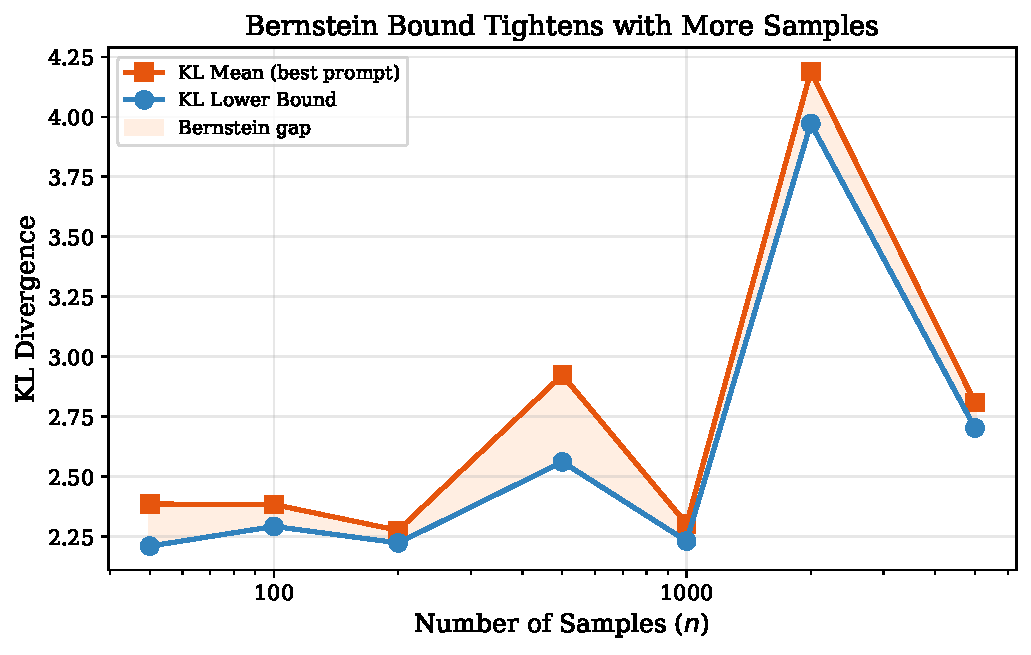
\includegraphics[width=\textwidth]{figures/fig3_sample_ablation.pdf}
  \centerline{\small (a) Sample count ablation}
\end{minipage}\hfill
\begin{minipage}[b]{0.48\textwidth}
  \centering
  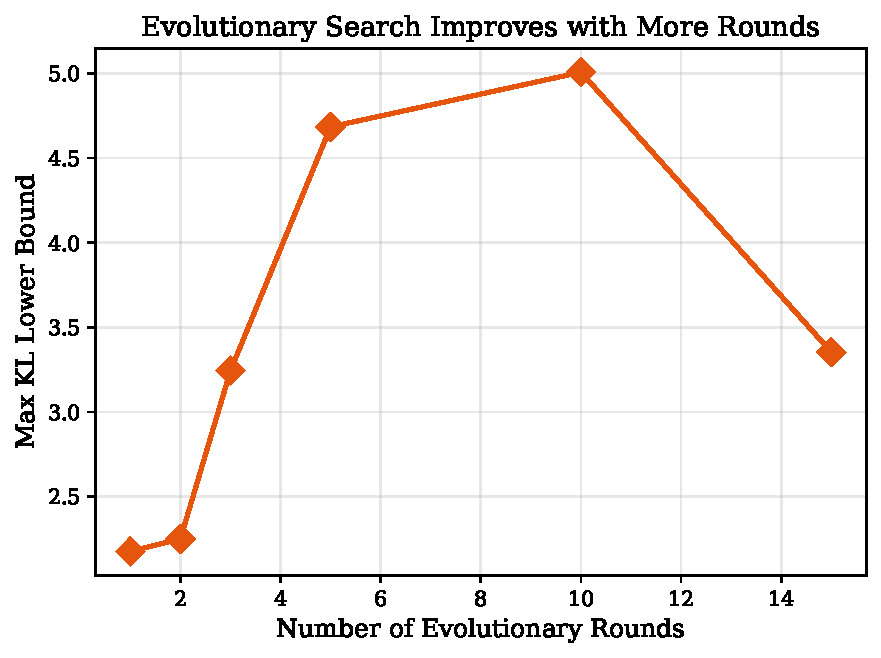
\includegraphics[width=\textwidth]{figures/fig4_round_ablation.pdf}
  \centerline{\small (b) Evolutionary round ablation}
\end{minipage}
\\[6pt]
\begin{minipage}[b]{0.48\textwidth}
  \centering
  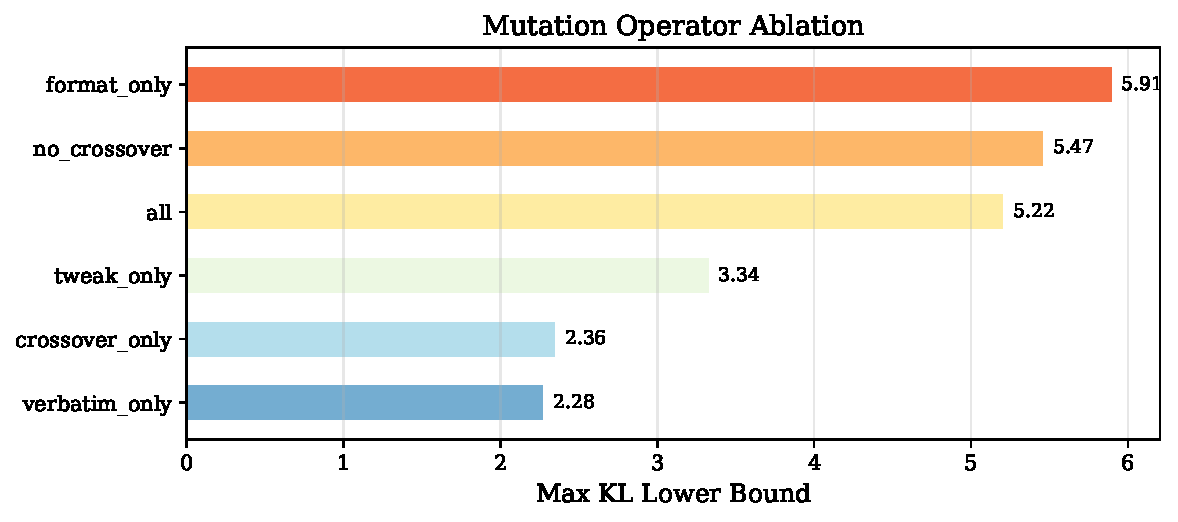
\includegraphics[width=\textwidth]{figures/fig5_mutation_ablation.pdf}
  \centerline{\small (c) Mutation operator ablation}
\end{minipage}\hfill
\begin{minipage}[b]{0.48\textwidth}
  \centering
  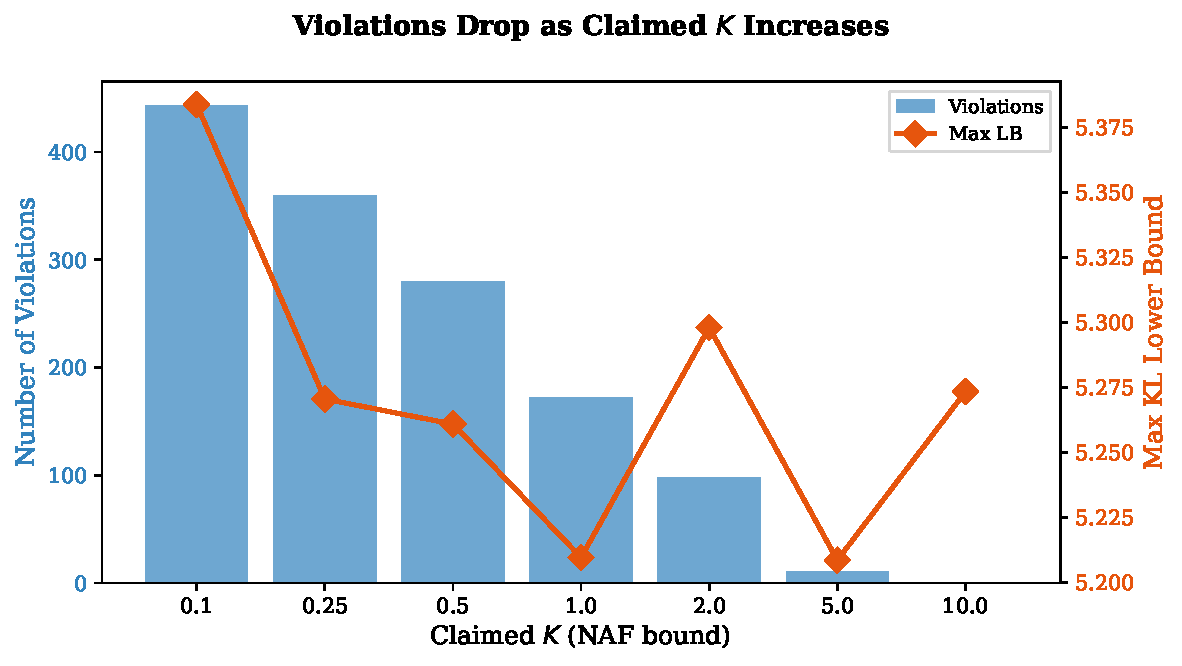
\includegraphics[width=\textwidth]{figures/fig6_k_threshold.pdf}
  \centerline{\small (d) $K$ threshold sweep}
\end{minipage}
\caption{Ablation studies. (a) Bernstein bound tightens with more samples. (b) Evolutionary search improves with more rounds. (c) Format-based mutations are most effective. (d) Violations decrease as claimed $K$ increases.}
\label{fig:ablations}
\end{figure}


%% ============================================================
\section{Discussion and Remaining Work}
\label{sec:discussion}
%% ============================================================

The early results show that the auditing framework works and that it gives meaningful numbers. A few things are still pending for the final report:
(i) scaling up to larger models (GPT-2 XL, Pythia-1B) on GPU;
(ii) auditing an actual NAF-compliant system---specifically anchored decoding \cite{he2026anchored}---and checking if the claimed $K$ really holds;
(iii) moving from token-level KL to sequence-level (addressing the limitation noted in assumption A5);
and (iv) using curated memorised passages from Carlini et al.\ \cite{carlini2021extracting} as seed prompts to stress-test the evolutionary search.

\paragraph{LLM disclosure.}
LLM Claude Opus was used in two ways: first, for coding assistance-implementing the Python framework, writing experiment configs, and producing figures; and second, for understanding the research papers. The project idea, experimental design, mathematical formulations, and choice of results are my own, and I independently verified every claim by running the experiments and reading the cited papers. The LaTeX has been edited and reviewed by me before submission.


%% ============================================================
% References
%% ============================================================

\begin{thebibliography}{12}

\bibitem{vyas2023naf}
N.~Vyas, S.~M.~Kakade, and B.~Barak.
\newblock On provable copyright protection for generative models.
\newblock In \emph{ICML}, 2023.

\bibitem{he2026anchored}
J.~He, J.~Hayase, W.-T.~Yih, S.~Oh, L.~Zettlemoyer, and P.~W.~Koh.
\newblock Anchored decoding: Provably reducing copyright risk for any language model.
\newblock \emph{arXiv preprint arXiv:2602.07120}, 2026.

\bibitem{jagielski2020auditing}
M.~Jagielski, J.~Ullman, and A.~Oprea.
\newblock Auditing differentially private machine learning.
\newblock In \emph{NeurIPS}, 2020.

\bibitem{nasr2023tight}
M.~Nasr, J.~Hayes, T.~Steinke, B.~Balle, F.~Tram\`{e}r, M.~Jagielski, N.~Carlini, and A.~Terzis.
\newblock Tight auditing of differentially private machine learning.
\newblock In \emph{USENIX Security}, 2023.

\bibitem{steinke2023one}
T.~Steinke, M.~Nasr, and M.~Jagielski.
\newblock Privacy auditing with one (1) training run.
\newblock In \emph{NeurIPS}, 2023.

\bibitem{pillutla2023auditing}
K.~Pillutla, G.~Andrew, P.~Kairouz, H.~B.~McMahan, A.~Oprea, and S.~Oh.
\newblock Unleashing the power of randomization in auditing differentially private {ML}.
\newblock In \emph{NeurIPS}, 2023.

\bibitem{maurer2009bernstein}
A.~Maurer and M.~Pontil.
\newblock Empirical {B}ernstein bounds and sample variance penalization.
\newblock \emph{arXiv preprint arXiv:0907.3740}, 2009.

\bibitem{carlini2021extracting}
N.~Carlini, F.~Tram\`{e}r, E.~Wallace, M.~Jagielski, A.~Herbert-Voss, K.~Lee, A.~Roberts, T.~Brown, D.~Song, U.~Erlingsson, A.~Oprea, and C.~Raffel.
\newblock Extracting training data from large language models.
\newblock In \emph{USENIX Security}, 2021.

\bibitem{shi2024bookmia}
W.~Shi, A.~Ajith, M.~Sakarvadia, A.~Agarwal, M.~Muez, D.~Marshall, and K.~Chard.
\newblock Detecting pretraining data from large language models.
\newblock In \emph{ICLR}, 2024.

\bibitem{pillutla2021mauve}
K.~Pillutla, S.~Swayamdipta, R.~Zellers, J.~Thickstun, S.~Welleck, Y.~Choi, and Z.~Harchaoui.
\newblock {MAUVE}: Measuring the gap between neural text and human text using divergence frontiers.
\newblock In \emph{NeurIPS}, 2021.

\bibitem{vinod2025invisibleink}
V.~Vinod, K.~Pillutla, and A.~Thakurta.
\newblock {InvisibleInk}: High-utility and low-cost text generation with differential privacy.
\newblock In \emph{NeurIPS}, 2025.

\bibitem{xie2024dpsynthtext}
C.~Xie, Z.~Lin, A.~Backurs, S.~Gopi, D.~Yu, H.~A.~Inan, H.~Nori, H.~Jiang, H.~Zhang, Y.~T.~Lee, et~al.
\newblock Differentially private synthetic data via foundation model {API}s 2: Text.
\newblock In \emph{ICML}, 2024.

\bibitem{bunsteinke2016cdp}
M.~Bun and T.~Steinke.
\newblock Concentrated differential privacy: Simplifications, extensions, and lower bounds.
\newblock In \emph{TCC}, 2016.

\end{thebibliography}


%% ============================================================
\newpage
\appendix
\section{Additional Experimental Results}
\label{app:additional}
%% ============================================================

\subsection{Model Pair Comparison Across Families}

Figure~\ref{fig:modelpairs} shows the full model pair comparison across all three families.
The sanity check (GPT-2 vs GPT-2) correctly yields zero KL, confirming the estimator is unbiased.
Evolutionary search outperforms random baselines for every non-trivial pair.

\begin{figure}[H]
\centering
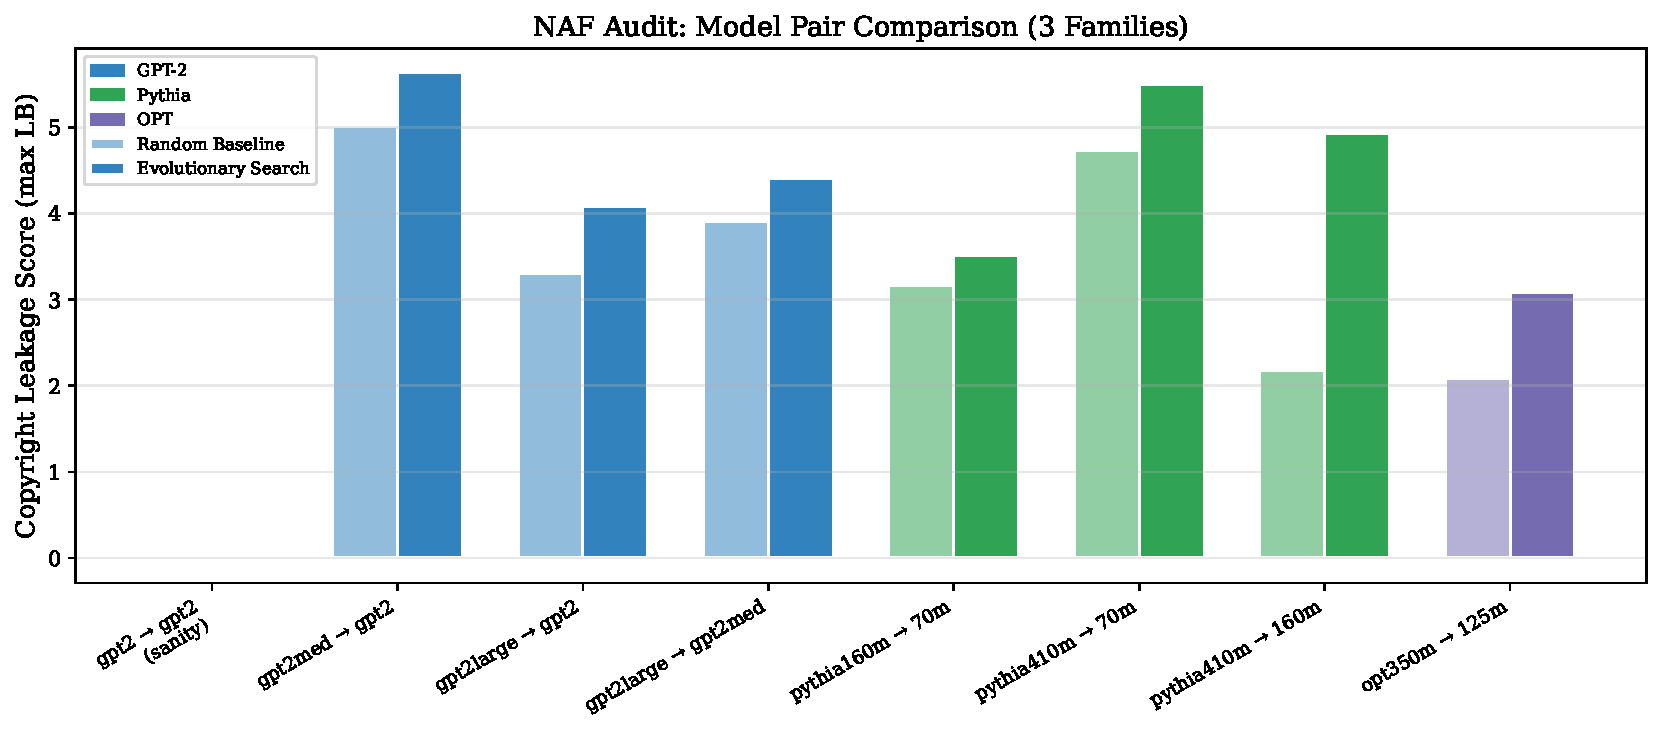
\includegraphics[width=0.78\textwidth]{figures/fig1_model_pairs.pdf}
\caption{Copyright Leakage Score across 8 model pairs from 3 families. Bars are coloured by family (blue = GPT-2, green = Pythia, purple = OPT). Evolutionary search consistently finds higher lower bounds than random.}
\label{fig:modelpairs}
\end{figure}

\subsection{Large-Scale Experiment}

Figure~\ref{fig:largescale} shows the distribution of KL lower bounds for 500 BookMIA prompts with 2000 samples and 10 rounds of evolutionary search.
The evolutionary method shifts the entire distribution of lower bounds upward and discovers prompts with substantially higher KL.

\begin{figure}[H]
\centering
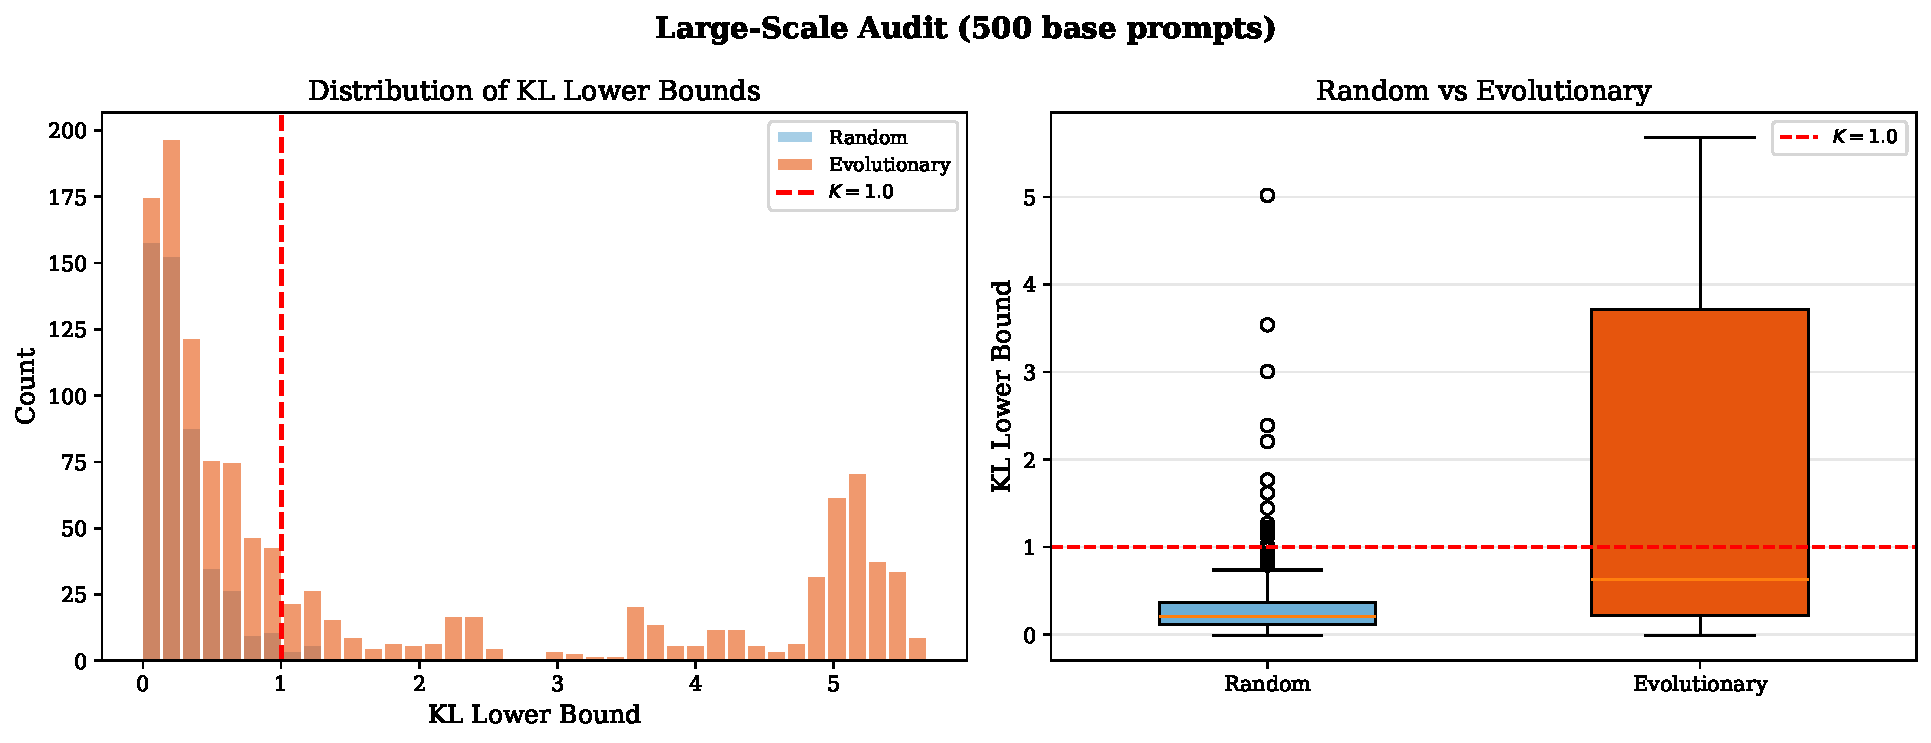
\includegraphics[width=0.78\textwidth]{figures/fig8_largescale.pdf}
\caption{Large-scale audit with 500 prompts. Left: histogram of KL lower bounds. Right: box plot comparison. The dashed red line marks $K = 1.0$.}
\label{fig:largescale}
\end{figure}

\subsection{Confidence Sweep and Experiment Overview}

Figure~\ref{fig:delta_and_summary} (left) shows the trade-off between confidence and tightness: lower $\delta$ (higher confidence) gives a looser lower bound, as expected from the $\ln(2/\delta)$ term in the Bernstein correction. Figure~\ref{fig:delta_and_summary} (right) gives a bird's-eye view of all 52 sub-experiments -red bars mark experiments with at least one violation, green bars mark those without.

\begin{figure}[H]
\centering
\begin{minipage}[b]{0.38\textwidth}
  \centering
  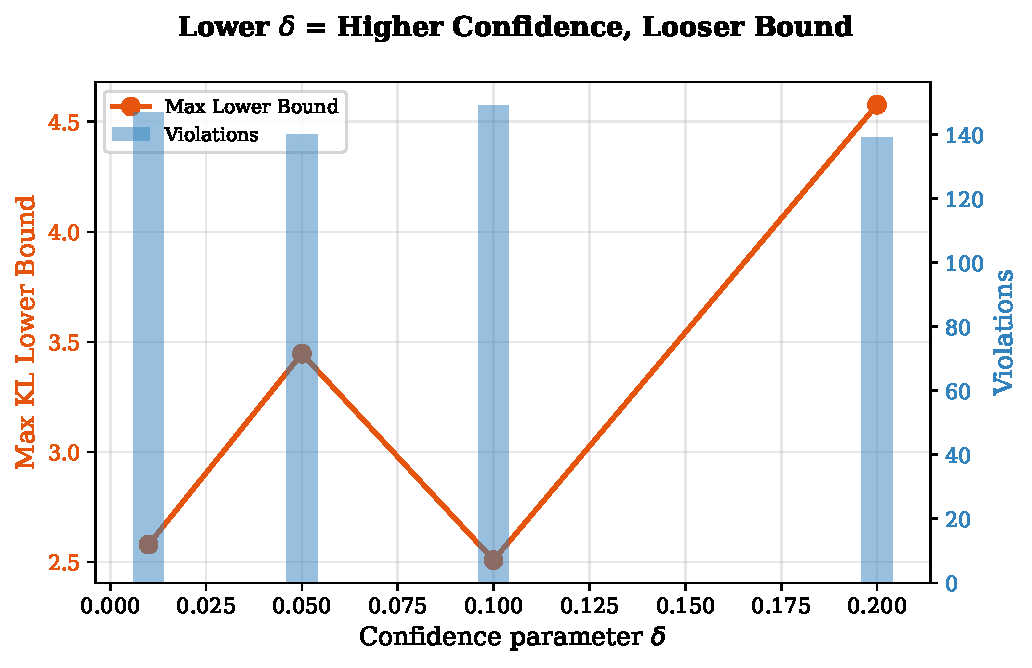
\includegraphics[width=\textwidth]{figures/fig7_delta_sweep.pdf}
  \centerline{\small (a) $\delta$ sweep}
\end{minipage}\hfill
\begin{minipage}[b]{0.60\textwidth}
  \centering
  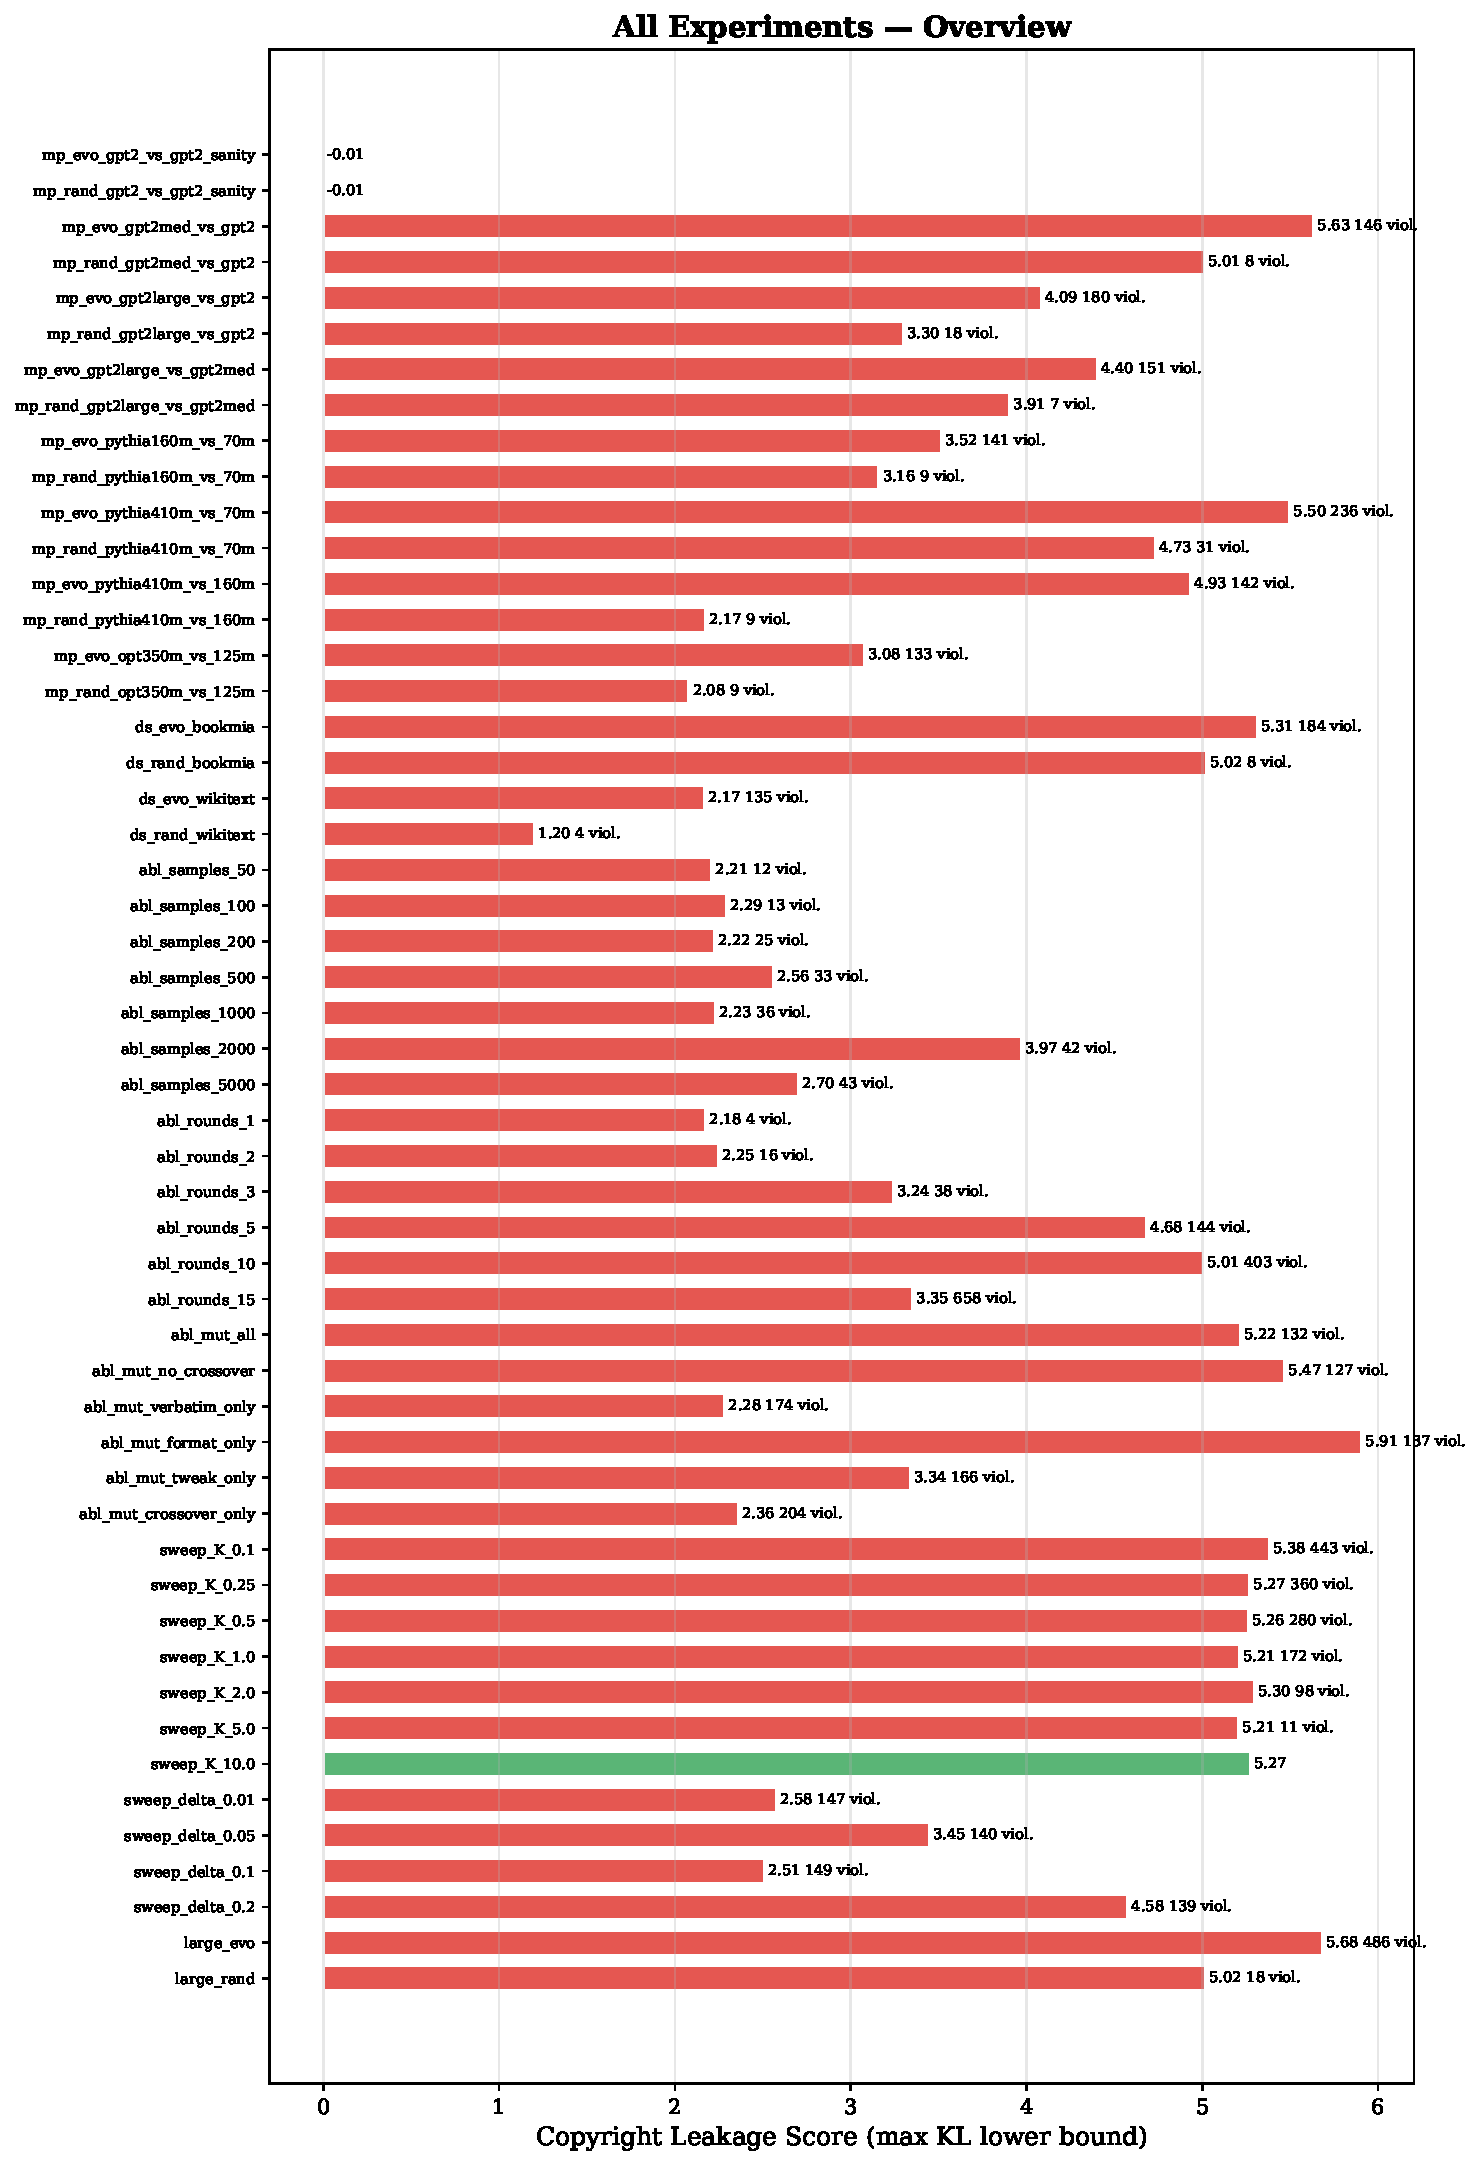
\includegraphics[width=\textwidth]{figures/fig9_summary.pdf}
  \centerline{\small (b) Overview of all 52 sub-experiments}
\end{minipage}
\caption{(a) Effect of $\delta$ on the lower bound. (b) Per-experiment violation status: red = at least one violation, green = none.}
\label{fig:delta_and_summary}
\end{figure}

\end{document}
